% \begin{figure*}[t]
%   \centering
%   \begin{minipage}{0.45\textwidth}
%     \centering
%     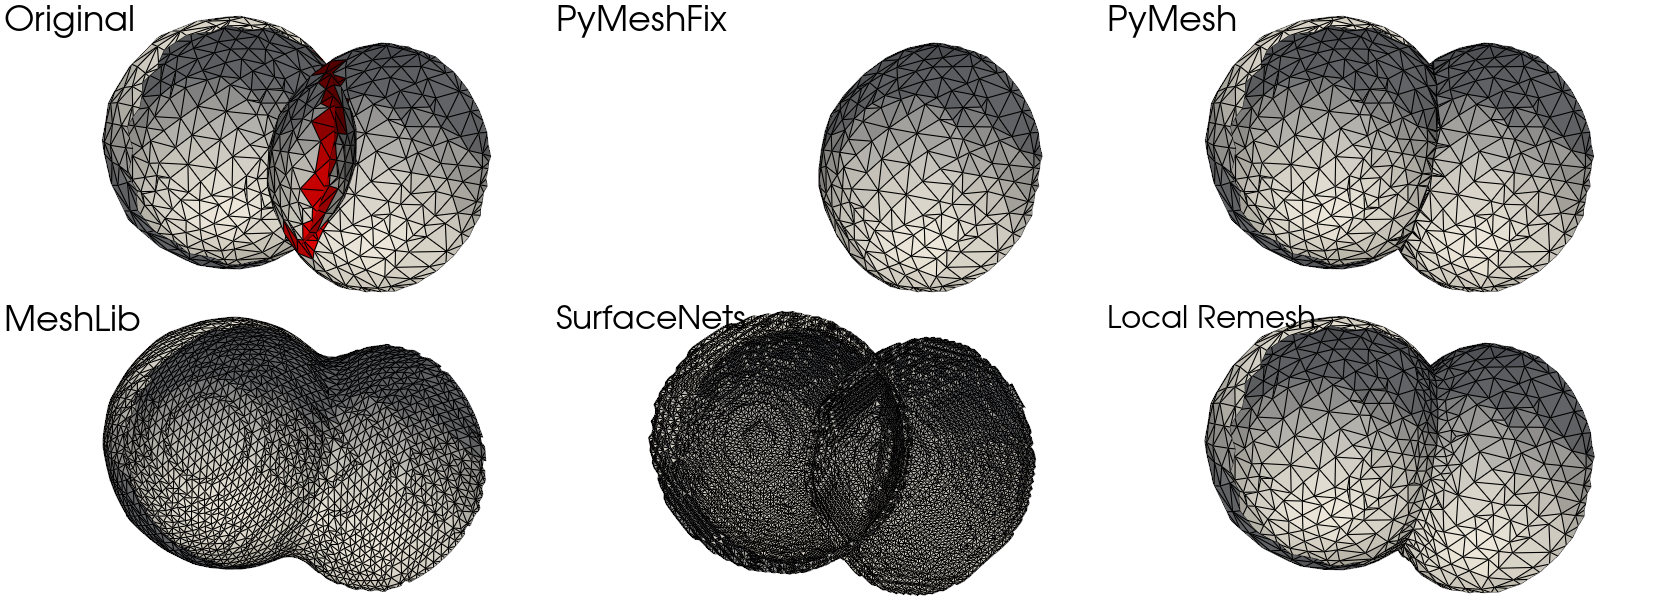
\includegraphics[width=\linewidth]{../figures/test_case1_inner.png}
%     % 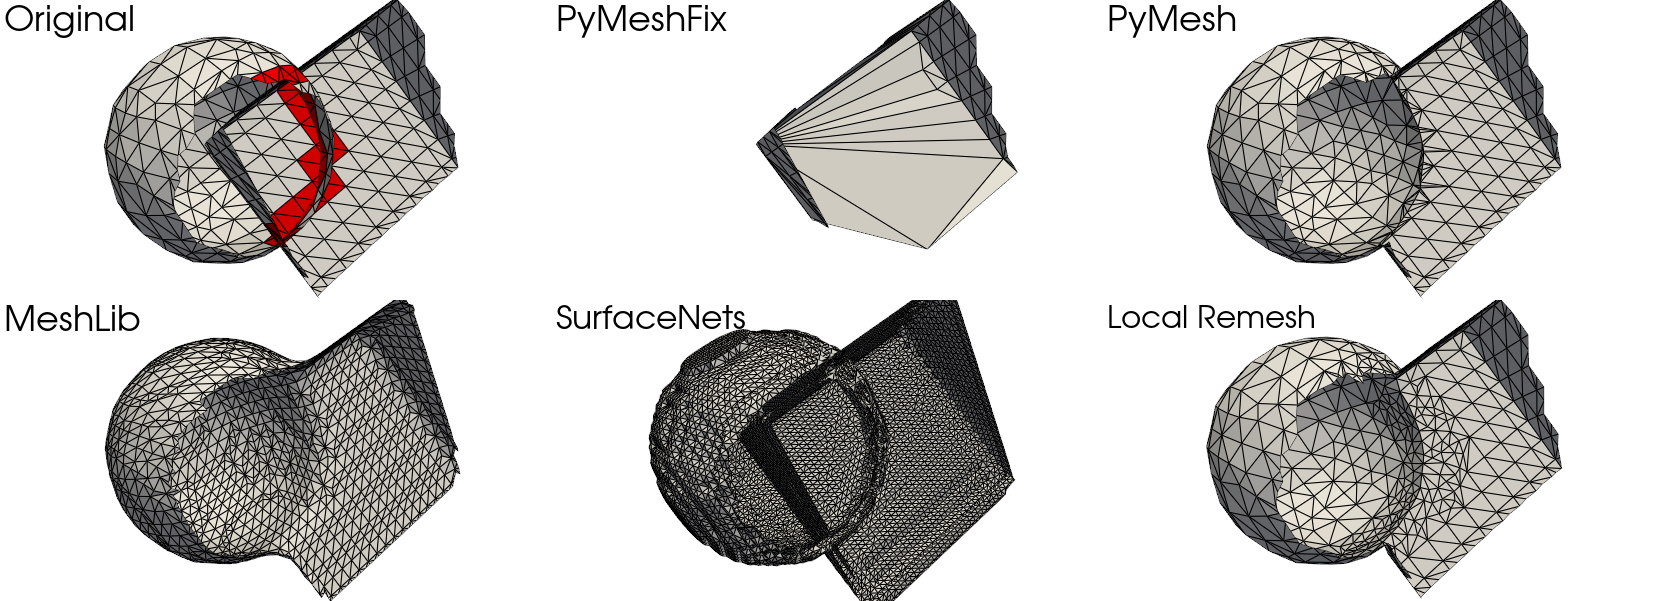
\includegraphics[width=\linewidth]{../figures/test_case3_inner.png}
%   \end{minipage}
%   \begin{minipage}{0.54\textwidth}
%     \centering
%     \renewcommand{\arraystretch}{0.45}
%     \small
%     \setlength{\tabcolsep}{1.2pt}
%     \begin{tabular}{lrrrrrr}
%         \toprule
%         \textbf{Metric} & Original & PyMeshFix & PyMesh & MeshLib & SurfaceNets & LocalRemesh \\
%         \midrule
%         No. vertices                & 952       & 476       & 917       & 15760      & 34766 & 937       \\
%         No. faces                   & 1896      & 948       & 1830      & 31516     & 73132 & 1870      \\
%         No. inters. faces  & 119       & 0         & 0         & 0        &  0  & 0         \\
%         Volume [m$^3$]                 & 7.08     & 3.57     & 6.61     & 6.61  & 6.96 & 6.61     \\
%         Area [m$^2$]                    & 22.57    & 11.37    & 19.08    & 18.91   & 48.12 & 19.08    \\
%         Aspect ratio       & 1.44     & 1.39     & 10.35    & 1.55    & \textbf{1.37}  & 1.44  \\
%         Condition          & 1.24     & \textbf{1.18}     & 10.07    & 1.29 & 1.20 & 1.24  \\
%         Max. angle [deg]          & 84.54    & 84.76    & 88.91    & 91.34 & \textbf{80.89}& 84.49  \\
%         Min. angle [deg]          & 41.62    & 41.91    & 37.70    & 37.50& \textbf{43.28}& 41.44  \\
%         Angle dev. [deg]    & 17.18    & 17.25    & 20.57    & 21.69& \textbf{14.79}& 17.18     \\
%         Scaled Jacobian    & 0.76     & 0.76     & 0.69     & 0.70& \textbf{0.79}& 0.75  \\
%         Displ. [m]      & NA       & 0.23     & \textbf{0.02} & 0.06  & 0.07& 0.03  \\
%         Intact vertices [\%]    & NA       & 50.00        & 84.03    & 0.00         & 0.00    & 77.00     \\
%         \bottomrule
%     \end{tabular}\par\vspace{5mm}

%     % \iffalse
%     % \begin{tabular}{lrrrrrr}
%     %     \toprule
%     %     \textbf{Metric} & Original & PyMeshFix & PyMesh & MeshLib & SurfaceNets & LocalRemesh \\
%     %     \midrule
%     %     No. vertices                & 1608      & 536       & 1576      & 26588& 61786 & 1564      \\
%     %     No. faces                   & 3204      & 1068      & 3148      & 53172& 129624 & 3124      \\
%     %     No. inters. face pairs  & 292       & 0         & 0         & 0        & 0     & 0         \\
%     %     Volume [m$^3$]                  & 11.96    & 3.99     & 11.02    & 11.02 & 11.60 & 11.01    \\
%     %     Area [m$^2$]                    & 36.60    & 12.20    & 29.38    & 29.08& 78.29 & 29.38    \\
%     %     Mean aspect ratio       & 1.33     & \textbf{1.33}     & 7.59   & 1.56& 1.41 & 1.37  \\
%     %     Mean condition          & 1.15     & \textbf{1.15}     & 7.33   & 1.30 & 1.24 & 1.18  \\
%     %     Mean max angle  [deg]         & 81.72    & 81.72    & 88.20    & 91.43 & \textbf{80.21}& 82.75  \\
%     %     Mean min angle  [deg]         & 41.22    & 41.22    & 36.63    & 37.58& \textbf{43.67}& 41.01  \\
%     %     Mean scaled Jacobian    & 0.76     & 0.76     & 0.67     & 0.70     & \textbf{0.79}& 0.75  \\
%     %     Mean displ. [m]       & NA       & 0.36     & \textbf{0.03}  & 0.06& 0.07& 0.04  \\
%     %     Mean angle dev. [deg]    & 15.73    & 15.73    & 20.16    & 21.80 & \textbf{14.35}& 16.37     \\
%     %     Intact vertices [\%]    & NA       & 33.33    & 80.35    & 0.00& 0.00& 70.65     \\
%     %     \bottomrule
%     % \end{tabular}\par\vspace{2mm}
%     % \fi

%     % \begin{tabular}{lrrrrrr}
%     %     \toprule
%     %     \textbf{Metric} & Original & PyMeshFix & PyMesh & MeshLib & SurfaceNets & LocalRemesh \\
%     %     \midrule
%     %     No. vertices                & 760       & 230       & 758       & 11064& 23773 & 860       \\
%     %     No. faces                   & 1512      & 456       & 1512      & 22124& 48932 & 1716      \\
%     %     No. inters. faces  & 99        & 0         & 0         & 0& 0 & 0         \\
%     %     Volume [m$^3$]                  & 11.59    & 6.95     & 10.85    & 10.817& 5.43& 10.84    \\
%     %     Area [m$^2$]                    & 34.64    & 25.12    & 29.92    & 29.30& 69.64 & 29.92    \\
%     %     Aspect ratio       & 1.39     & 2.21     & 2.13     & 1.52 & \textbf{1.40} & 1.42  \\
%     %     Condition          & 1.18     & 1.87     & 1.86     & 1.27 & \textbf{1.18} & 1.20  \\
%     %     Max. angle [deg]          & 86.46    & 96.10    & 90.45    & 90.82& \textbf{85.88}& 86.31  \\
%     %     Min. angle [deg]          & 41.66    & 35.01    & 38.04    & 37.51& \textbf{41.32}& 40.87  \\
%     %     Angle dev. [deg]    & 17.91    & 24.37    & 20.88    & 21.07& \textbf{17.65}& 18.07     \\
%     %     Scaled Jacobian    & 0.76     & 0.65     & 0.70     & 0.70 & \textbf{0.76}& 0.75  \\
%     %     Displ. [m]       & NA       & 0.31     & \textbf{0.03}     & 0.08& 0.11 & 0.04  \\
%     %     Intact vertices [\%]    & NA       & 30.26    & 86.71    & 0.00& 0.00& 79.74     \\
%     %     \bottomrule
%     % \end{tabular}
%   \end{minipage}
%   \caption{\textbf{Merging two neighboring meshes.} Visual (left) and quantitative (right) comparison of mesh quality for the original and repaired meshes in test case 1 (top) and 2 (bottom) using five different repair methods. Figures show the inside of each mesh with intersections marked in red. In the tables, all metrics from aspect ratio to angle deviation are the mean value across the entire output mesh. For each metric, the value of the best-performing mesh is shown in bold.}
%   \label{fig:wide_combo}
% \end{figure*}

\section{Merging neighboring meshes}
We selected the five methods described below based on their usability, high performance, popularity, and the uniqueness of their functionalities.
\textbf{PyMeshFix}: A mesh-based repair. It first removes self-intersecting triangles and then fills the resulting holes. We called the function \texttt{pymeshfix.clean\_from\_arrays()} from PyMeshFix, a Python wrapper for MeshFix, developed by Attene \cite{attene2010lightweight}.
\textbf{PyMesh}: A mesh-based repair. It fixes self-intersections by subdividing intersecting facets, adding new vertices and edges as needed. We called the fuction \texttt{pymesh.compute\_outer\allowbreak\_hull()} from PyMesh, which internally calls a function to resolve self-intersections during execution. The libgil engine runs in the background of this function call \cite{jacobson2018libigl}.  \textbf{MeshLib}: A voxel-based repair. MeshLib is an open-source 3D mesh library designed for geometry processing. We called \texttt{mrmeshpy.fixSelf\allowbreak Intersections()} for self-intersection resolution. For voxelization, the voxel size was set to a quarter of the median edge length. 
\textbf{SurfaceNets}: A voxel-based repair. In her study, Frisken extended 3D SurfaceNets to generate high-resolution and smooth 3D meshes from multi-labeled segmented volumes \cite{frisken2022surfacenets}. It enables the generation of a mesh with sharp boundaries preserved from the input after applying surfacing methods. In this evaluation, we used the original C++ implementation. The voxel size was set to a quarter of the median edge length here as well. 
\textbf{LocalRemesh}: A mesh-based repair. We implemented a method that locally remeshes intersecting areas. As mentioned earlier, a common challenge faced by many mesh-based repair methods that involve subdividing facets is the generation of ill-shaped triangles in the output mesh, which negatively impacts mesh quality. To address this, this method ensures that even after subdivision, any ill-shaped triangles are corrected through local remeshing. This was implemented using existing mesh libraries including trimesh. 


Test Case 1 consists of two intersecting spheres. The left side of Figure \ref{fig:teaser} shows the original state and the state after repair for all five methods. 
The various methods can be seen to produce structurally different results. However, all resulted in no intersections, indicating that each method achieved geometric correctness. 

When looking at our mesh quality metrics, SurfaceNets produced a mesh with better overall mesh quality, indicating that the repaired mesh has well-shaped triangles on its surface. The evaluation results also highlight strong performance of Meshlib. This can be attributed to the fact that both SurfaceNets and MeshLib repair self-intersections through global remeshing. The mesh gets a new surface during the process, which results in high-quality triangles. However, it is important to note that the performance of global remeshing methods depends on the voxel size. In this evaluation, the voxel size was set to a quarter of the median edge length. If we had chosen the voxel size to be larger or smaller, the performance could have been better or worse, changing how these methods compare to the others. 

In reviewing structural integrity, some methods successfully preserved the original geometry, while others did not.  PyMeshFix produced a mesh with one of the components missing after the repair, because the algorithm only keeps the largest component of the mesh and discards the rest. This would not be an issue with a self-intersecting mesh such as a brain that has intersecting gyri. However, in cases where intersections are due to submeshes, such as the two components shown here, the output would greatly deviate from the original geometry. PyMesh and SurfaceNets produced output meshes that have inner boundaries between the original components, with SurfaceNets leaving the original boundaries unchanged and PyMesh merging the two intersecting sections into one. These options may or may not be a viable solution depending on the application. For example, a volume mesh algorithm that fills triangular meshes with tetrahedral elements may not be able to process such a mesh. MeshLib and LocalRemesh created meshes without inner components, such that the resulting mesh forms an outer hull of the original mesh. For the purpose of creating a finite element volume mesh, such solutions are ideal.

In terms of geometric correctness and structural integrity, the repair algorithm of PyMesh can be considered stable. However, when we focus on mesh quality, the repaired meshes raise concerns for practical applications. Figure \ref{fig:sol1-analysis} shows a closer look at the repaired mesh from Test Case 1. As can be seen in the figure, the repaired sections consist of ill-shaped triangles. In such a geometry, both large and small angles could have detrimental effects on finite element modeling. The LocalRemesh method is based on PyMesh, but performs additional local remeshing to eliminate the ill-shaped triangles produced by PyMesh. These differences are reflected in the calculated metrics as PyMesh having 1) smaller differences between the original and output mesh (smaller displacement and higher percentage of intact vertices), and 2) worse results in all triangle quality metrics (maximum and minimum angle, angle deviation, aspect ratio, condition and scaled Jacobian). This example demonstrates the importance of carefully evaluating quality metrics, and choosing a mesh repair method based on metrics that reflect the desired output.

Further test cases are presented in the supplemental material. % and the meshes can be viewed interactively online.
The produced results are structurally similar to what we saw for Test Case 1. In addition to basic geometric shapes, we also assessed these methods with a brain surface mesh created from a T1-weighted MRI scan of a 28-year-old male. Figure 1 in the supplemental material shows the results. For complicated cases like this, there is a need to be more careful, as the resulting differences are less visually obvious compared to simple ones.


\begin{figure}[h]
    \centering
    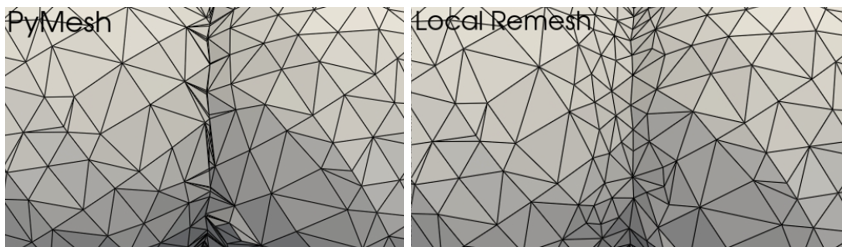
\includegraphics[width=0.90\linewidth, height=2.4cm]{../figures/3.png}
     \caption{\textbf{Closeup of LocalRemesh vs PyMesh.} Both methods repaired the intersections between two neighboring meshes, but LocalRemesh produced a result of much higher quality.}
     \label{fig:sol1-analysis}
\end{figure}